%%%%%%%%%%%%%%%%%%%%%%%%%%%%%%%%%%%%%%%%%%%%%%%%%%%
%% LaTeX book template                           %%
%% Author:  Amber Jain (http://amberj.devio.us/) %%
%% License: ISC license                          %%
%%%%%%%%%%%%%%%%%%%%%%%%%%%%%%%%%%%%%%%%%%%%%%%%%%%

\documentclass[a4paper,11pt]{book}
\usepackage[T1]{fontenc}
\usepackage[utf8]{inputenc}
\usepackage{lmodern}
%%%%%%%%%%%%%%%%%%%%%%%%%%%%%%%%%%%%%%%%%%%%%%%%%%%%%%%%%
% Source: http://en.wikibooks.org/wiki/LaTeX/Hyperlinks %
%%%%%%%%%%%%%%%%%%%%%%%%%%%%%%%%%%%%%%%%%%%%%%%%%%%%%%%%%
\usepackage{hyperref}
\usepackage{graphicx}
\usepackage[english]{babel}
\usepackage[a4paper,top=2cm,bottom=2cm,left=2cm,right=2cm]{geometry}
\usepackage{lscape}
\usepackage{caption}
\usepackage{amsmath}
\usepackage{listingsutf8}
\usepackage{listings}
\usepackage{float}
\usepackage{amsmath}
\usepackage{subfig}
\usepackage{xcolor}
\usepackage{textcomp}
\usepackage{wrapfig}
\usepackage{rotating}
\usepackage{epstopdf}
\usepackage{commath}

\definecolor{codegreen}{rgb}{0,0.6,0}
\definecolor{codegray}{rgb}{0.5,0.5,0.5}
\definecolor{codepurple}{rgb}{0.58,0,0.82}
\definecolor{backcolour}{rgb}{0.95,0.95,0.92}

\lstdefinestyle{mystyle}{
	backgroundcolor=\color{backcolour},   
	commentstyle=\color{codegreen},
	keywordstyle=\color{magenta},
	numberstyle=\tiny\color{codegray},
	stringstyle=\color{codepurple},
	basicstyle=\ttfamily\footnotesize,
	language = C++,
	%frameround=fttt,
	%frame = trBL,
	firstnumber = last,
	breakatwhitespace=false,         
	breaklines=true,                 
	captionpos=b,                    
	keepspaces=true,                 
	numbers=left,                    
	numbersep=5pt,                  
	showspaces=false,                
	showstringspaces=false,
	showtabs=false,                  
	tabsize=2
}

\lstset{style=mystyle}

\captionsetup{tableposition=top,figureposition=bottom,font=small}
%%%%%%%%%%%%%%%%%%%%%%%%%%%%%%%%%%%%%%%%%%%%%%%%%%%%%%%%%%%%%%%%%%%%%%%%%%%%%%%%
% 'dedication' environment: To add a dedication paragraph at the start of book %
% Source: http://www.tug.org/pipermail/texhax/2010-June/015184.html            %
%%%%%%%%%%%%%%%%%%%%%%%%%%%%%%%%%%%%%%%%%%%%%%%%%%%%%%%%%%%%%%%%%%%%%%%%%%%%%%%%
\newenvironment{dedication}
{
   \cleardoublepage
   \thispagestyle{empty}
   \vspace*{\stretch{1}}
   \hfill\begin{minipage}[t]{0.66\textwidth}
   \raggedright
}
{
   \end{minipage}
   \vspace*{\stretch{3}}
   \clearpage
}

%%%%%%%%%%%%%%%%%%%%%%%%%%%%%%%%%%%%%%%%%%%%%%%%
% Chapter quote at the start of chapter        %
% Source: http://tex.stackexchange.com/a/53380 %
%%%%%%%%%%%%%%%%%%%%%%%%%%%%%%%%%%%%%%%%%%%%%%%%
\makeatletter
\renewcommand{\@chapapp}{}% Not necessary...
\newenvironment{chapquote}[2][2em]
  {\setlength{\@tempdima}{#1}%
   \def\chapquote@author{#2}%
   \parshape 1 \@tempdima \dimexpr\textwidth-2\@tempdima\relax%
   \itshape}
  {\par\normalfont\hfill--\ \chapquote@author\hspace*{\@tempdima}\par\bigskip}
\makeatother

%%%%%%%%%%%%%%%%%%%%%%%%%%%%%%%%%%%%%%%%%%%%%%%%%%%
% First page of book which contains 'stuff' like: %
%  - Book title, subtitle                         %
%  - Book author name                             %
%%%%%%%%%%%%%%%%%%%%%%%%%%%%%%%%%%%%%%%%%%%%%%%%%%%

% Book's title and subtitle
\title{
	
\includegraphics[width=0.7\textwidth]{Immagini/UniBg.png}
	\\ \Huge \textbf{Progetti di Informatica III A} \\ Università degli Studi di Bergamo \\ \huge A.A. 2019/2020}
% Author
\author{\\ \textsc{Piffari Michele - 1040658}}

\begin{document}
	
	\frontmatter
	\maketitle
	
	%%%%%%%%%%%%%%%%%%%%%%%%%%%%%%%%%%%%%%%%%%%%%%%%%%%%%%%%%%%%%%%%%%%%%%%%
	% Auto-generated table of contents, list of figures and list of tables %
	%%%%%%%%%%%%%%%%%%%%%%%%%%%%%%%%%%%%%%%%%%%%%%%%%%%%%%%%%%%%%%%%%%%%%%%%
	\tableofcontents
	\listoffigures	
	\mainmatter
	
	
	\mainmatter
	\chapter{I - Cyclone}
	\section{Introduzione}
Il progetto è stato realizzato e testato in linguaggio C, per poi essere portato in Cyclone.

Il porting è stato effettuato manualmente ed è consistito principalmente nella
ridefinizione dei tipi puntatore, che rappresentato il cavallo di battaglia di Cyclone
nell’assicurare la type safety.
Si è provato anche il porting semi-automatico, come supporto per la traduzione manuale.

Cyclone è un dialetto safe del C che permette di prevenire diversi tipi di errori e problemi di
sicurezza molto comuni in C come \textbf{buffer overfow, stringhe non terminate e dangling pointers}.
Per ottenere questi risultati si è andato ad aggiunger il garbage collector, che solleva il programmatore dal dover esplicitamente deallocare la memoria con le chiamate free(), riducendo la possibilità di incorrere in dangling pointer o di memoria non deallocata al termine del suo utilizzo.

Altra caratteristica importante di Cyclone sono i qualificatori dei puntatori che meglio
specificano i possibili valori assunti dai puntatori e aggiungono controlli sull'utilizzo degli stessi.

\section{Descrizione del progetto}

L'applicazione scritta in C e successivamente tradotta in Cyclone, consiste in un piccolo programmino in grado di leggere dati da un file, parsarli, fornendo poi una funzionalità di ricerca sui dati contenuti al suo interno.

Nello specifico si è pensato di inserire questa applicazione nell'area break dell'università: infatti, in concomitanza con la macchinettà del caffè gestita in \textit{ASMETA} e il distributore di energy drink prodotto in \textit{Scala}, ho pensato di introdurre un sistema per gestire cartoline, da spedire ai propri cari per gli studenti fuori sede.

Nello specifico è stata realizzata un'interfaccia in grado di funzionare in questo modo:
\begin{itemize}
	\item L'applicazione legge i dati da un file \textit{.txt} in cui sono contenute una serie di cartoline descritte da
	\begin{itemize}
		\item Mittente
		\item Destinatario
		\item Località da cui è stata spedita
	\end{itemize}
	\item Ognuna della informazioni che caratterizza ogni singola cartolina è divisa per mezzo di un carattere delimitatore ("|") che permette alla funzione di \textit{tokenize} di andare ad assegnare le corrette informazioni ad ogni singola cartolina
	\item Una volta letto il file in ingresso, che potrebbe rappresentare l'insieme di tutte le cartoline relativo ad un account su una specifica piattaforma online per la gestione delle cartoline, l'interfaccia permette di eseguire una ricerca:
	\begin{itemize}
		\item \textit{BY SENDER}
		\item \textit{BY RECEIVER}
		\item \textit{BY PLACE}
	\end{itemize}
	stampando poi le cartoline trovate (qualora ce ne fossero).
\end{itemize}

\section{Costrutti Cyclone}
In questa piccola applicazione sono stati due i costrutti principali di Cyclone che sono stati utilizzati:
\begin{itemize}
	\item \textbf{Puntatori}: Cyclone permette l'utilizzo di normali puntatori con le seguenti modifiche rispetto a C
	\begin{itemize}
		\item Controlla se il puntatore è nullo ad ogni de-reference dello stesso (previene \textbf{Segmentation Fault})
		\item Cast vietato da int a puntatore (previene \textbf{Out of Bounds})
		\item Aritmetica dei puntatori vietata (previene \textbf{Buffer Oveflow ~ Overrun e Out of Bounds})
	\end{itemize}
	Ogni puntatore ha inoltre una serie di annotazioni che specificano come deve essere trattato;
	ogni annotazione inizia con un carattere @. 
	
	\item \textbf{Regioni}: vedi sezione ~\ref{sec:regions}
\end{itemize}
\subsection{Puntatori @fat e @thin}
I puntatori sono di default \textbf{@thin}, ovvero non sono in grado di controllare dinamicamente il rispetto dei limiti (bounds) dell’array.

I puntatori \textbf{@fat} (definiti in modo abbreviato con il carattere ?) effettuano invece tale controllo ogni volta che viene utilizzata l’aritmetica dei puntatori.
Essi possono essere pensati come una struttura (struct), per cui i fat pointer permettono l’aritmetica sia in avanti sia all’indietro, con la garanzia di non eccedere i limiti dell’array, come si vede in figura ~\ref{fig:fatStruct}.

\begin{figure}[h]
	\centering
	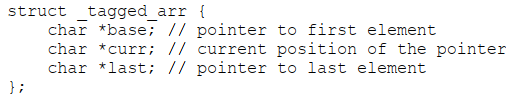
\includegraphics[width=0.5\textwidth]{Immagini/FatPointerStruct.png}
	\caption{@fat pointer visto come una Struct}
	\label{fig:fatStruct}
\end{figure}

Questa tipologia di puntatori, è stata usata diffusamente all'interno del codice Cyclone, sopratutto nella funzione di \textit{tokenize} dove si è ritenuto opportune sfruttare il fatto che i \textit{fat} pointer contengano l'informazione sulla lunghezza, accessibile tramite il comando \textit{numelts}.

\subsection{Puntatori @nullable e @notnull}
\subsubsection{@nullable}
I puntatori sono di default \textbf{@nullable}, ovvero possono assumere valore NULL. Tali puntatori si possono definire anche esplicitamente con *@nullable. 
I puntatori fat possono essere solo @nullable: un puntatore @fat@notnull può essere nullo,

Questa tipologia di identificatori per i puntatori sono stati utilizzati nella fase di apertura del file \textit{.txt}: come si vede in figura ~\ref{fig:nullable}, non  uso di puntatore \textit{@notnull} per garantire le gestione del caso in cui non si riesca ad aprire il file di testo, tramite un print di errore.

\begin{figure}[h]
	\centering
	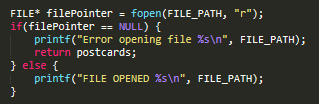
\includegraphics[width=0.5\textwidth]{Immagini/NullablePointerFile.png}
	\caption{Gestione pointer nullable}
	\label{fig:nullable}
\end{figure}

\subsubsection{@notnull}
I puntatori @notnull non possono invece essere nulli, ovvero non è possibile assegnare loro il
valore NULL. Essi possono essere definiti in modo abbreviato con il carattere @.
I puntatori non nulli sono sicuramente i più utilizzati, sia perché non introducono l’overhead
del controllo di non-nullità (che viene garantita a compile-time), sia perché nella quasi totalità
dei casi un puntatore è utilizzato per operare sull’oggetto puntato e non per verificare se tale
oggetto esiste, quindi si dà per scontato che esso esista.

Questa tipologia di puntatore è stata largamente utilizzata nper quanto riguarda le stringhe, relative alla struttura \textit{postcard}.

\subsection{Regioni}
\label{sec:regions}
Per evitare dangling pointers, Cyclone impone che ogni puntatore dichiari in quale area della
memoria punti. L’area (region) in cui punta può essere un particolare record di attivazione
sullo stack, lo heap o una regione di stack allocata dinamicamente. Ogni puntatore può puntare
solo a regioni che hanno una vita uguale o più lunga di quella della regione dichiarata; ad
esempio, un puntatore allo heap può puntare solo allo heap, un puntatore al record di
attivazione di una funzione può puntare a quel record, ai record dei chiamanti della funzione o
allo heap, ma non può puntare a record di funzioni chiamate

Per indicare esplicitamente una regione, si deve annotare il puntatore con @region(`r) o
@effect(`r) o semplicemente `r, dove r è il nome di un’opportuna regione o un semplice
segnaposto. `H rappresenta lo heap.
	\chapter{II - C++}
	\section{Descrizione del progetto}
Per quanto riguarda il progetto realizzato in cpp si è pensato, piuttosto che realizzare un applicativo "funzionale" (approccio seguito per gli altri 3 progetti), di andare a realizzare una libreria per il calcolo numerico, che consiste in due moduli principali:
\begin{itemize}
	\item Matrici
	\item Applicativo dimostrativo
\end{itemize}

In particolare sono state sviluppate alcune funzionalità algebriche base come \textbf{somma} e \textbf{sottrazione} elemento per elemento di una matrice: l'espressività del C++ ha permesso di rendere questa libreria del tutto generica, permettendo quindi di realizzare matrici composte da elementi di qualsiasi tipo, tramite l'utilizzo dei \textbf{templates generici}.

\section{Gerarchia delle classi}
Come si vede nell'\textit{UML Class Diagram} in figura ~\ref{fig:UMLClassDiagram}, la libreria presenta una classe base principale, \textit{Number}, che rappresenta un numero il quale può essere un numero di tipo \textit{Addable} o \textit{Subtractable}, che offrono rispettivamente un metodo e un operatore per realizzare la somma e la sottrazione.
\begin{figure}[h]
	\centering
	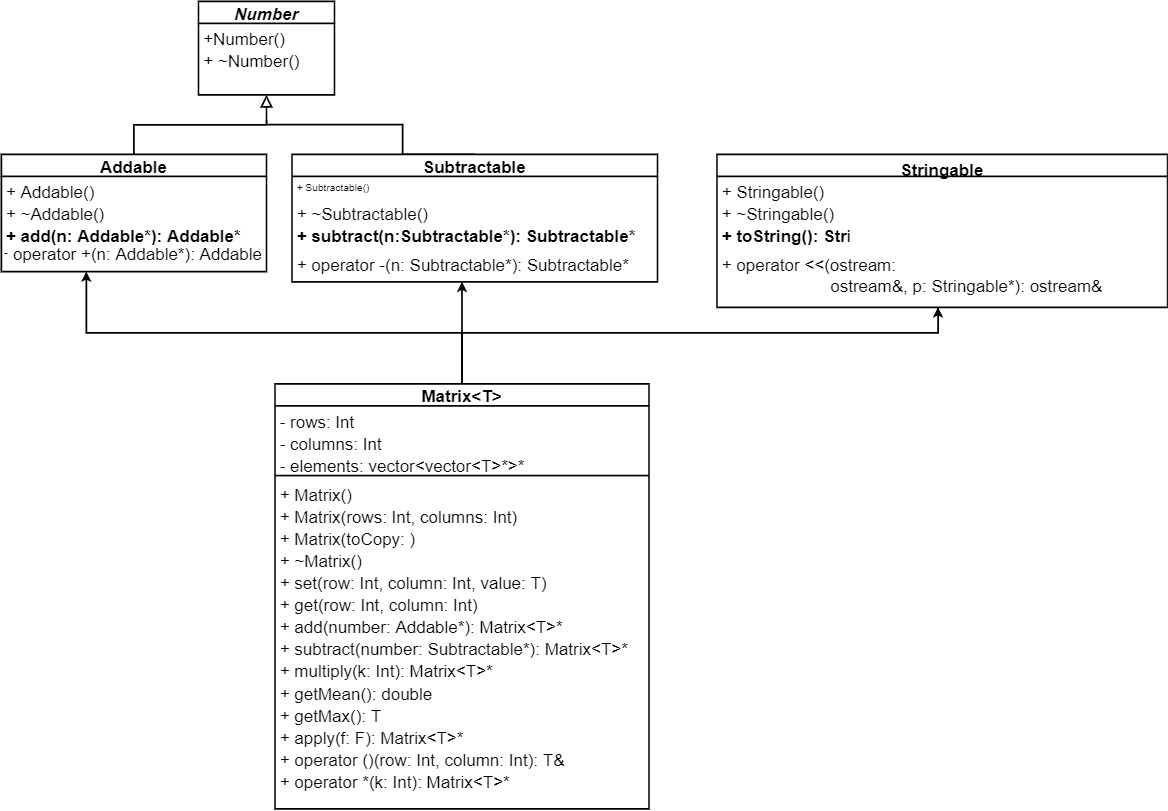
\includegraphics[width=0.7\textwidth]{Immagini/ClassDiagram.jpg}
	\caption{UML class diagram}
	\label{fig:UMLClassDiagram}
\end{figure}

\section{Multiple inheritance}
Nella gerarchia delle classi sopra esposta, è stato necessario utilizzare l’ereditarietà multipla
nei due diversi contesti tipici: 
\begin{itemize}
	\item \textbf{implementazione di interfacce}
	\item \textbf{ereditarietà multipla classica}
\end{itemize}

\textbf{Il C++ non fa distinzioni sostanziali tra queste due tipologie, ma la differenza concettuale è
notevole, tanto che altri linguaggi (come Java) i quali permettono di implementare più interfacce ma non di ereditare di più classi.}

La prima tipologia consiste nel derivare una classe da al più una classe base “non pure virtual”.
Le altre classi base devono essere l’equivalente delle interface Java, ovvero devono essere
classi astratte (\textit{Abstract Base Classes} - ABCs) in cui tutte le member functions sono
pure virtual.

\textbf{Questa tipologia di eredità è stata utilizzata per derivare da Stringable}.

La seconda tipologia di eredità è stata invece utilizzata per andare a modellizzare il rapporto tra una matrice e quelle che sono le strutture relative a \textbf{Number}, come si vede nella figura ~\ref{fig:MultipleInerithance}.

\begin{figure}[h]
	\centering
	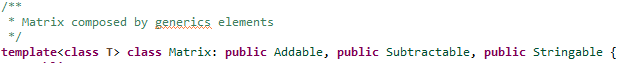
\includegraphics[width=0.6\textwidth]{Immagini/MultipleInerithance.png}
	\caption{Esempio di eredità multipla della classe \textit{Matrix}}
	\label{fig:MultipleInerithance}
\end{figure}

\section{Diamond inheritance}
Un aspetto problematico dell’ereditarietà multipla (specialmente quando si attua una doppia ereditarietà da due classi diverse, la quale è una peculiarità del C++) è la
possibilità di generare una \textbf{gerarchia a diamante}.

Essa si verifica quando, come si vede nella figura ~\ref{fig:DiamondProblem}, una generica classe D eredita da due classi B e C che hanno un antenato in comune A. In questo caso c'è un'ambiguità su quale “versione” dell'antenato deve essere ereditata da D: quella di B o quella di C?

\begin{figure}[h]
	\centering
	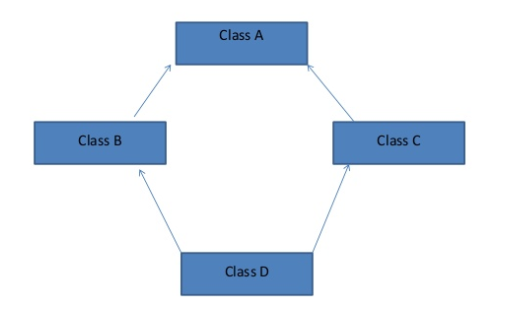
\includegraphics[width=0.3\textwidth]{Immagini/DiamondProblem.png}
	\caption{Diamond problem}
	\label{fig:DiamondProblem}
\end{figure}

Un modo di risolvere il problema in C++ è dichiarare, nelle classi B e C, un'\textbf{eredità virtuale} da A, specificandolo direttamente nella dichiarazione, come fatto nelle classi \textbf{Addble} e \textbf{Subtractable} (figura ~\ref{fig:VirtualInerithance}).

\begin{figure}[h]
	\centering
	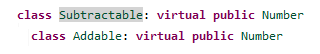
\includegraphics[width=0.5\textwidth]{Immagini/VirtualInerithance.png}
	\caption{Virtual Inerithance nelle classe \textit{Addable} e \textit{Subtractable}}
	\label{fig:VirtualInerithance}
\end{figure}

\section{Costruttori e distruttori}
\subsection{Costruttori}
La libertà di poter utilizzare oggetti all'interno delle applicazioni scritte in C++, si incontra però con la necessità di andare a compiere due operazioni preliminari:
\begin{itemize}
	\item Allocare la memoria dei membri dell'oggetto in esame;
	\item Inizializzate i membri.
\end{itemize}
Queste operazioni sono svolte da una particolare funzione membro detta \textbf{costruttore}, il cui nome coincide con quello della classe e non presenta alcun valore di ritorno.

In C++ un costruttore che non accetta argomenti, o in cui tutti gli argomenti sono opzionali, è detto \textbf{costruttore di default} ed è possibile sovraccaricare questo metodo, fornendo quindi diverse alternative. E' comunque sempre buona norma andare a realizzare l'overloading del costruttore di default, perchè esso ha dei limiti come il fatto che il valore predefinito per il tipo di ogni dato membro può dipendere dal compilatore utilizzato, e quindi non essere deterministico.

\subsection{Distruttori}
Dal lato opposto, il \textbf{distruttore} si occupa del compito di rilasciare tutte le risorse associate ad un oggetto, quando finisce la lifetime dell'oggetto stesso: infatti il distruttore viene invocato per tutte le variabili automaticamente ogni volta che viene raggiunta la fine del loro \textit{scope} e tutte le volte che le variabili dinamiche vengono deallocate con la parola chiave \textit{delete}.

In particolare, come per il costruttore, anche il distruttore presenta una firma particolare, ovvero presenta lo stesso nome della classe solamente per il fatto che è preceduto dal simbolo ~ (\textit{tilde}); anch'esso, come il costruttore, non presenta alcun valore di ritorno, e in più non presenta parametri (motivo per cui non può essere sovraccaricato).

Inoltre se non viene esplicitamente incluso nella dichiarazione della classe, il distruttore viene generato automaticamente dal compilatore. In questo caso tuttavia, l’unica risorsa rilasciata è la memoria occupata dall’oggetto: se alcuni dei suoi dati membro sono delle reference, o se l’oggetto fa uso di altre risorse (file o altre interfacce di I/O), potrebbe essere necessario svolgere delle operazioni per il loro corretto rilascio.

\subsection{Implementazione nell'applicazione}
Queste caratteristiche sono state sfruttate per quanto riguarda gli oggetti della classe \textit{Matrix}.

Per quanto riguarda la costruzione degli oggetti di tipo \textit{Matrix} sono stati sovraccaricati i costruttori di default, con 2 alternative differenti: come si vede in figura ~\ref{fig:matrixInit}

\begin{figure}[h]
	\centering
	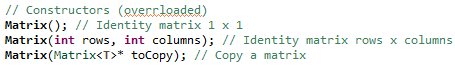
\includegraphics[width=0.8\textwidth]{Immagini/MatrixConstructors.png}
	\caption{Costruttori classe \textit{Matrix}}
	\label{fig:matrixInit}
\end{figure}

In particolare si ha che:
\begin{itemize}
	\item Il primo costruttore rappresenta il costruttore di default, ed è stato implementato per fornire un'inizializzazione "custum" (e non di default del compilatore) ai membri della classe. Esso va a creare una matrice identità di dimensioni 1x1;
	\item Il secondo costruttore invece va a inizializzare i mebri della classe \textit{Matrix} in maniera tale da ricreare una matrice di dimensioni \textit{rows x columns} (parametri passati in input al costruttore);
	\item L'ultimo overriding del costruttore di \textit{Matrix} permette di inizializzare un nuovo oggetto \textit{Matrix} tramite un altro oggeto di tipo \textit{Matrix}.
\end{itemize}

Per quanto riguarda il distruttore (figura ~\ref{fig:matrixDeInit}) sono due gli aspetti da porre ini evidenza:
\begin{itemize}
	\item é stato definito \textit{virtual} in maniera tale che venissero chiamati anche i distruttori delle superclassi;
	\item esso si occupa, come si vede nella relativa implementazione, di andare a liberare la memoria allocata per la struttura contenete gli elementi della matrice: per fare ciò s è fatto uso di un iteratore sulle righe della matrice, in maniera tale da andare poi a liberare ogni elemento della colonna.
\end{itemize}

\begin{figure}[h]
	\centering
	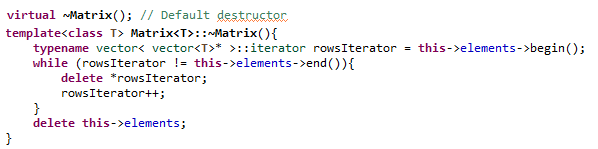
\includegraphics[width=0.8\textwidth]{Immagini/MatrixDestructors.png}
	\caption{Firma e implementazione del distruttore della classe \textit{Matrix}}
	\label{fig:matrixDeInit}
\end{figure}

\section{Overloading particolari}
Nella nostra libreria, su consigli di altri studenti, siamo andati a ridefinire alcuni operatori, per renderli più "personalizzati".
\subsection{Overloading di cout<<}
Tra gli operatori che risulta utili sovraccaricare c'è "<<", il quale è utilizzato nella libreria standard per inviare dati agli oggetti \textit{ostream} (flussi in output): è stato quindi possibile personalizzare, in maniera facile e diffusa, la tipologia di log aggiungendo, come si vede in figura ~\ref{fig:CoutRedef}, un print personalizzato, per distinguere così il log della libreria da quello di sistema classico.

\begin{figure}[h]
	\centering
	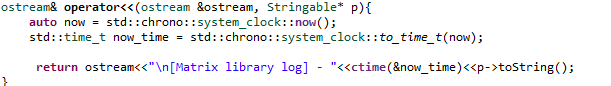
\includegraphics[width=0.8\textwidth]{Immagini/CoutRedefinition.png}
	\caption{Ridefinizione dell'operatore di stream}
	\label{fig:CoutRedef}
\end{figure}

\subsection{Overloading di ()}
L'operatore () è leggeremente diverso dagli altri, in quanto è possibile interpretarlo in due modi, a seconda che compaiano in un l-value ("get") o in un r-value ("set").

In C++ è possibile sovraccaricare gli operatori in modo che si comportino in maniera diversa a seconda della posizione esattamente come accade con gli array.

\begin{figure}[h]
	\centering
	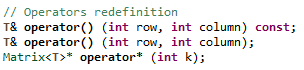
\includegraphics[width=0.5\textwidth]{Immagini/MatrixOperatorsRedef.png}
	\caption{Ridefinizione degli operatori nella classe \textit{Matrix}}
	\label{fig:MatrixOperatorRedef}
\end{figure}

Nella nostra applicazione siamo andati a ridefinire appunto l'operatore (), come si vede in figura ~\ref{fig:MatrixOperatorRedef}, in particolare:
\begin{itemize}
	\item  la presenza del simbolo \textbf{$\&$} subito dopo il valore ritornato indica che ci sono\textbf{ due definizioni diverse dello stesso operatore}.
	\item il modificatore \textbf{const} indica invece che la\textbf{ prima ridefinizione è quella da usare se l'operatore sta a sinistra} (\textit{l-value}) del simbolo di assegnamento.
\end{itemize}
Un esempio di applicazione della redefinizione dell'operatore (), li si possono vedere in figura ~\ref{fig:OperatorExamples}.

\begin{figure}[h]
	\centering
	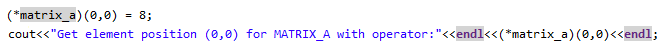
\includegraphics[width=0.8\textwidth]{Immagini/OperatorExample.png}
	\caption{Esempio di utilizzo della redefinizione degli operatori}
	\label{fig:OperatorExamples}
\end{figure}

\section{Templates}
Un metodo più potente per il riutilizzo del codice è fornito dai templates. 

Essi costituiscono uno “schema” di classe che poi verrà realizzato concretamente sostituendo ai tipi parametrici i tipi effettivi dichiarati dagli utilizzatori.

A differenza del linguaggio Java, ogni differente realizzazione del template costituisce un tipo
a sé stante e senza alcuna relazione con gli altri: in Java si può avere una gerarchia di tipi
derivati dallo stesso template.

In C++ invece ogni realizzazione di un template viene concretizzata tramite codice
indipendente, portando quindi ad un file eseguibile di dimensioni maggiori. Inoltre, per fornire
vincoli in modo esplicito come in Java, si deve ricorrere a una “pseudo-ereditarietà”.

Questa flessibilità offerta dai templates, è stata utilizzata nella stesura della classe \textit{Matrix}.

\section{Standard Template Library}
La libreria STL del C++ mette a disposizione una serie di contenitori parametrici, che quindi
possono contenere oggetti di tipo arbitrario. Fornisce inoltre iteratori che permettono di visitare
tali contenitori e algoritmi per manipolarne gli elementi.

Uno dei contenitori più semplici è \textit{vector}, una classe che permette di gestire collezioni di oggetti ordinati come un array.

I vantaggi del vector sul semplice array sono diversi, tra cui la gestione automatica della
memoria e la presenza di diversi metodi per le operazioni più comuni quali l'inserimento di un
nuovo valore.

La classe Matrix utilizza un vector per memorizzare gli elementi della matrice ed essendo
parametrica di parametro T, utilizza un \textit{vector<vector<T>>}.
\subsection{STL - Iterator}
Tra le altre funzionalità messe a disposizione da vector e dagli altri contenitori in STL ci sono gli
iteratori, che costituiscono il modo standard di accedere agli elementi nel contenitore stesso. Gli
iteratori si comportano in modo simile a semplici puntatori (ad esempio ammettono l'operatore ++),
anche se in realtà sono più flessibili e possono essere utilizzati anche con le liste.

\begin{figure}[h]
	\centering
	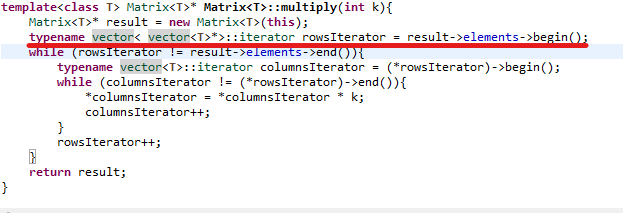
\includegraphics[width=0.7\textwidth]{Immagini/Stl_Iterator.png}
	\caption{STL - Iterator}
	\label{fig:Iterator}
\end{figure}

\subsection{STL - Algorithm}
La libreria STL mette a disposizione anche degli algoritmi generici e riutilizzabili per operare sui contenitori.

Tali algoritmi sono implementati tramite funzioni template che si possono includere nei propri file tramite la direttiva di include.

Un esempio di algoritmo è la funzione \textit{for-each()}, che applica una funzione parametro a tutti gli
elementi di un contenitore.

\begin{figure}[h]
	\centering
	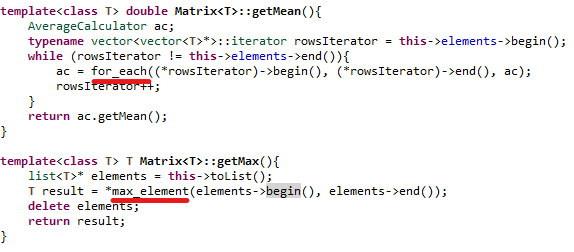
\includegraphics[width=0.7\textwidth]{Immagini/Stl_Algorithm.png}
	\caption{STL - Algorithm}
	\label{fig:Algoritm}
\end{figure}
	\chapter{III - Energy drink vending machine con Scala}
	\section{Descrizione del progetto}
Il progetto scritto in Scala prevede di andare ad affiancare, alla macchinetta del caffè gestita in ASMETA, un distributore automatico di bevande energetiche.

In particolar modo si è progettato un sistema con queste specifiche:
\begin{itemize}
	\item Ogni distributore automatico può essere impostato, in fase di installazione, per funzionare in una lingua piuttosto che in un'altra: nel codice è gestitata solamente la possibilità di introdurre distirbutori automatici in \textbf{lingua italiana} e in \textbf{lingua inglese}.
	\item Ogni ditributore è riconosciuto tramite un identificativo univoco (\textbf{ID}).
	\item Questa tipologia di distributori sono in grado di erogare le seguenti bevande energetiche (\textit{energy drink}):
	\begin{itemize}
		\item \textbf{RedBull};
		\item \textbf{Monster};
		\item \textbf{Gatorade};
		\item \textbf{Italian} (particolare energy drink \textit{made in Italy}, che NON viene erogato da distributori in lingua inglese).
	\end{itemize}
	Ognuno di questi prodotti sarà caratterizzato dai seguenti campi descrittivi:
	\begin{itemize}
		\item \textbf{Prezzo};
		\item \textbf{Volume} (espresso in cl);
		\item\textbf{Data di scadenza};
		\item Insieme di \textbf{tags}, che permettono di esprimere le caratteristiche e gliusi principali di ogni tipologia di energy drink (ovviamente, ogni lattina di RedBull, per esempio, avrà lo stesso insieme di tags).
		\item \textbf{Valore nutrizionale} indicato teramite tre possibili step
		\begin{itemize}
			\item \textbf{Ipercalorico}
			\item \textbf{Normocalorico}
			\item \textbf{Ipocalorico}
		\end{itemize}
	\end{itemize}
\end{itemize}

Ogni distributore andrà ad offrire le seguenti funzionalità:
\begin{itemize}
	\item \textbf{Acquisto dei prodotti} disponibili, \textbf{regalando i prodotti scaduti}: in particolare la macchinetta sarà in grado di fornire resto esatto al cliente (oppure tutta la somma di denaro inserita nel caso di prodotto scaduto).
	\item \textbf{Stampa dell'elenco dei prodotti disponibili} all'interno del distirbutore, unitamente al \textbf{numero di pezzi disponibili}, come si vede in figura ~\ref{fig:AvailableProducts}.
	\begin{figure}[h]
		\centering
		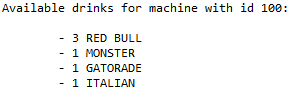
\includegraphics[width=0.4\textwidth]{Immagini/ShowVendingMachine.png}
		\caption{Prodotti disponibili}
		\label{fig:AvailableProducts}
	\end{figure}
	\item Possibilità di \textbf{cercare un prodotto tramite tag}, per poter così trovare l'energy drink più adatto ad ogni specifica evenienza
	\item \textbf{Aggiunta di lattine} di energy drink all'interno del distributore.
\end{itemize}

\section{Costrutti utilizzati}
\begin{itemize}
	\item Traits (sezione ~\ref{sec:traits});
	\item Comando \textit{filter} (sezione ~\ref{sec:filter})
	\item Match e Sealed (sezione ~\ref{sec:match_sealed})
\end{itemize}

\newpage
\section{Gerarchia delle classi e trait}
\label{sec:traits}
Nella applicazione realizzata sono stati realizzata due gerarchie facendo uso dei \textit{\textbf{trait}}: i trait in Scala corrispondono alle interfaccie in Java, ovvero permettono di definire la firma di ogni classe che ne implementa la struttura.

Nel nostro caso abbiamo due strutture gerarchiche, gestite tramite traits, mostrate con un grafo ad "albero" nell'immagine seguente (figura ~\ref{fig:classi&traits}).

\begin{figure}[h]
	\centering
	\subfloat[][\emph{Energy drink}]
	{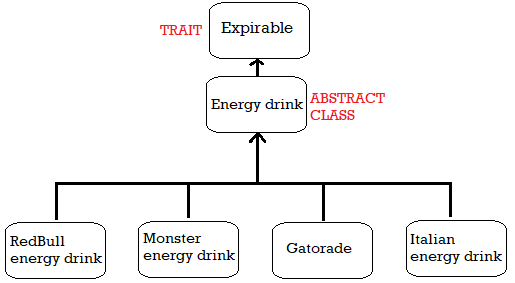
\includegraphics[width=.45\textwidth]{Immagini/EnergyDrink.png}} \quad
	\subfloat[][\emph{Expirable trait}]
	{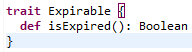
\includegraphics[width=.35\textwidth]{Immagini/ExpirableTrait.png}} \\
	\subfloat[][\emph{Vending machine}]
	{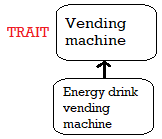
\includegraphics[width=.25\textwidth]{Immagini/VendingMachine.png}} \quad
	\subfloat[][\emph{Vending machine trait}]
	{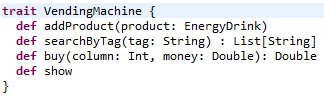
\includegraphics[width=.45\textwidth]{Immagini/VendingMachineTrait.png}}
	\caption{Classi e trait}
	\label{fig:classi&traits}
\end{figure}

Il primo albero gerarchico rappresenta la struttura che "governa" l'insieme dei possibili energy drink: ogni energy drink astratto eredita da \textit{Expirable} la possibilità di "scadere", che, grazie all'\textit{override} implementa direttamente nell'interfaccia astratta, dato che è uguale per ogni tipologia di energy drink concreta.

Il secondo albero gerarchico invece rappresenta l'appartenenza dell'unica tipologia di distributori trattati in questa applicazione (quelli di energy drink), ad un'interfaccia comune a tutte le possibili tipologie di distributori.

\newpage
\section{Filter}
\label{sec:filter}
Per quanto riguarda la funzionalità di ricerca delle bevande in base ai tag, è stata utile l'istruzione \textit{object oriented} \textit{filter}: in questo modo l'utente, in base alle diverse necessità (per esempio: studio intenso), può cercare l'energy drink più adatto.

Il comando di filter è utile nel momento in cui si vogliono filtrare gli elementi di una certa collezione (lista, array, vettore etc), andando a crearne una nuova contenente solamente gli elementi che rispettano il criterio di filtraggio definito in maniera custom (questo criterio è passato sotto forma di \textit{closures}, ovvero una funzione definita localmente "\textit{al volo}").

Nella nostra applicazione siamo andati a filtrare l'elenco dei tag di ogni prodotto: il filtraggio è stato pensato per mantenere solamente i tag contenenti al loro interno il tag cercato dall'utente tramite tastierino di input.

\begin{figure}[h]
	\centering
	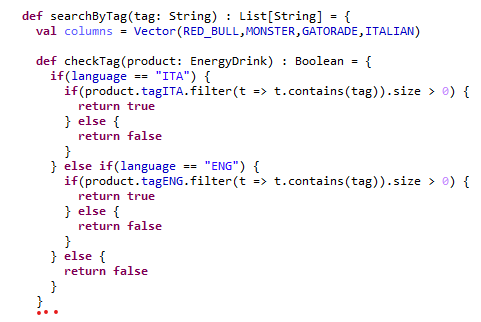
\includegraphics[width=0.55\textwidth]{Immagini/Filter.png}
	\caption{Utilizzo comando \textit{filter}}
	\label{fig:filter}
\end{figure}

\begin{figure}[h]
	\centering
	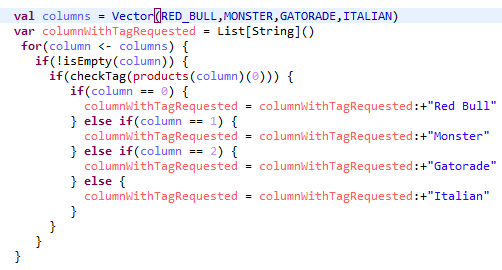
\includegraphics[width=0.55\textwidth]{Immagini/RicercaTag.png}
	\caption{Ricerca del tag su ogni possibile prodotto con \textit{checkTag}}
	\label{fig:filterSearch}
\end{figure}

Come si vede in figura ~\ref{fig:filter}, in base alla tipologia di lingua con cui il distributore è stato impostato, si va a cercare, \textbf{per ogni prodotto disponibile} (figura ~\ref{fig:filterSearch}), nei rispettivi tag, solamente quelli che contengono la parola chiave cercata dall'utente.

In particolare, se il risultato dell'operazione di filter è un vettore con una lunghezza maggiore di 0, significa che il prodotto in esame soddisfa il tag cercato, e quindi può essere mostrato all'utente. 

Questa operazione di filtraggio viene poi ripetuta per ogni tipologia di prodotto disponibile, ovvero per ogni colonna (dato che ogni prodotto ha lo stesso set di tags).

Una volta effettuato il filtraggio \textbf{ho considerato solamente i prodotti il cui risultato dall'operazione di filter non fosse un vettore vuoto}: questo corrisponde infatti al prendere solamente i prodotti che contengono il tag cercato, notificando poi all'utente la loro tipologia, tramite una stampa a display.

\section{Expression oriented programming}
\label{sec:match_sealed}
\subsection{Match}
Il \textit{pattern match} rappresenta una struttura per verificare il valore assunto da una variabile, tramite un pattern: si tratta in sostanza di una versione leggermente più potente del construtto \textit{switch} di Java.

Nell'applicazione si è pensato di andare ad utilizzare il \textit{pattern matching} in due situazioni:
\begin{itemize}
	\item \textit{Pattern guard}: nell'andare a definire se un prodotto è considerabile come normo, ipo o iper calorico, si è fatto uso di un pattern guard, sfruttando anche la potenzialità aggiuntiva di poter aggiungere una condizione dopo il pattern, tramite la dicitura \textit{if<boolean expression>}, che permette di rendere più specifico ogni singolo case.
	\item \textit{Matching on classes}: per la funzionalità di aggiunta di nuovi prodotti all'interno del distributore automatico, si era pensato di utilizzare un \textit{pattern match} per poter distinguere la tipologia specifica del prodotto aggiunto. Alla fine la scelta è però ricaduta sull'utilizzo del comando \textit{isInstanceOf}.
\end{itemize}
\subsection{Sealed}
Classi e traits possono essere segnati come \textit{sealed}: questo significa che tutti i sotto tipi devono essere dichiarati e implementati all'interno dello stesso file, garantendo che tutti i sottotipi siano conosciuti e noti già in fase di compilazione, prevenendo quindi errori nel nostro codice.


In questo modo, unendo l'utilizzo di classi \textit{sealed} con il \textit{pattern match}, siamo in grado di garantire \textit{type safety}.
Infatti questa struttura permette di garantire il fatto che i \textit{match cases} utilizzati saranno tutti esaustivi: questo grazie al fatto il compilatore conosce in anticipo tutte le possibili implementazioni, dato che sono implementate tutte nello stesso file.

\begin{figure}[h]
	\centering
	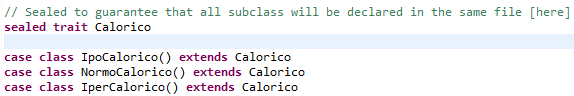
\includegraphics[width=0.5\textwidth]{Immagini/Sealed.png}
	\caption{Sealed}
	\label{fig:sealed}
\end{figure}

	\chapter{IV - Coffe Machine con ASM}
	\section{Descrizione del progetto}
Per quanto riguarda la parte di ASM  \textit{ASM} si è deciso di riprendere un esempio visto in classe (e durante le pause), ovvero quello relativo alla \textit{\textbf{Coffee machine}}, che affiancherà il distributore di bevande energetiche progettato in Scala.
In particolare si è definito l'applicazione su una serie di specifiche, quali:
\begin{itemize}
	\item Il distributore modellato può preparare diversi tipi di bevande (caffè, cappuccino etc), ognuna delle quali è preparata con diverse quantità di ingredienti (acqua, caffè, latte etc) i quali vengono consumati dagli utenti e reintegrati dal manutentore.
	\item Il distributore accetta pagamenti solamente in moneta tramite l'inserimento di denaro nell'apposita fessura.
	\item Il distributore è in grado di fornire il resto (anche se non sempre in modo esatto)
	\item Quando tutte le bevande sono esaurite, il distributore va fuori servizio, in attesa che gli ingredienti vengano aggiunti dal manutentore, il quale può inoltre prelevare o inserire monete dal distributore, sempr etenendo conto del vincolo di capacità del vano porta monete
\end{itemize}
	

\section{Macchina a stati}
La ASM è basata su una sottostante macchina a stati finiti, mostrata in figura ~\ref{fig:StateMachine}, che definisce i principali stati e transizioni del distributore. 
\begin{figure}[h]
	\centering
	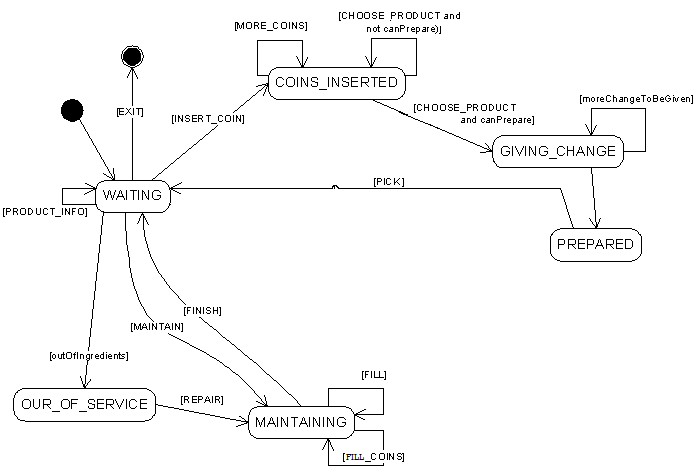
\includegraphics[width=0.8\textwidth]{Immagini/FSM.png}
	\caption{Macchina a stati}
	\label{fig:StateMachine}
\end{figure}
La ASM permette di estendere questa FSM introducendo un concetto aumentato di “stato”, che comprende anche funzioni dinamiche, modificando le quali si possono memorizzare informazioni aggiuntive.
In particolare, è stato possibile memorizzare informazioni su:
\begin{itemize}
	\item Quantità di ingredienti residui
	\item Monete possedute dal distributore
	\item Credito dell'utente attuale
\end{itemize}

\section{Eventi}
La ASM sviluppata modella un sistema event-driven, ovvero un sistema in cui le transizioni da uno stato all’altro sono perlopiù scatenate da input dell’utente, mentre di solito la macchina si trova ferma in uno stato, in attesa di tali eventi.
Nel codice della ASM questi eventi sono denominati action; ad ogni stato corrispondono una o più azioni che l’utente può compiere quando la macchina è in quello stato, le quali sono codificate come elementi di un dominio enumerativo, i quali essendo identificativi univoci, non possono essere duplicati, come si vede in figura ~\ref{fig:actionASM}.

\begin{figure}[h]
	\centering
	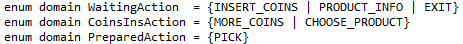
\includegraphics[width=0.8\textwidth]{Immagini/ActionASM.png}
	\caption{Action che implicano un possibile cambio di stato}
	\label{fig:actionASM}
\end{figure}

La caratteristica event-driven del sistema si è riflessa nella ASM, infatti le regole (\textit{rules}) implementate possono essere suddivise in due categorie:
\begin{itemize}
	\item  regole che attendono il verificarsi di un’azione (qui chiamate event management rules) e poi eseguono le corrette regole di transizione (transition rules)
	\item regole di transizione che verificano la guardia della transizione e, se verificata, eseguono gli update opportuni
\end{itemize}
	
In linea di massima, ad ogni stato corrisponde una \textit{event management rule}, mentre ad ogni arco (transizione) corrisponde una \textit{transition rule}.

\section{Domini}
Sono stati introdotti un dominio enumerativo per gli stati della FSM, uno per ciascun insieme di eventi (ciascun insieme contiene gli eventi validi per uno stato), ovvero quelli relativi alle possibili azioni eseguibili in ogni specifico stato, ed uno relativo alla tipologia di ingredienti utilizzati (figura ~\ref{fig:enumDomain})

\begin{figure}[h]
	\centering
	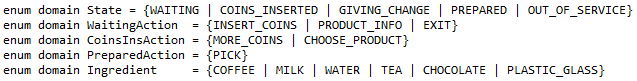
\includegraphics[width=0.8\textwidth]{Immagini/EnumDomain.png}
	\caption{Domini enumerativi}
	\label{fig:enumDomain}
\end{figure}

Sono stati introdotti anche un dominio statico concreto per i tagli di monete riconosciuti dal distributore (rappresentati in centesimi) e un dominio astratto per i prodotti disponibili.

\section{Controlled - static - monitored functions}
\subsection{Controlled}
Le funzioni in figura ~\ref{fig:notMonitored}, rappresentano funzioni non-monitored così definite:
\begin{figure}[h]
	\centering
	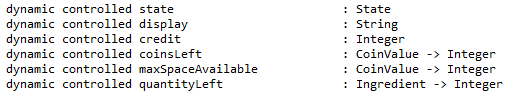
\includegraphics[width=0.8\textwidth]{Immagini/DynamicController.png}
	\caption{Funzioni non monitored}
	\label{fig:notMonitored}
\end{figure}

Si vede come le prime tre funzioni rappresentino delle funzioni 0-arie, ovvero delle variabili.

Le ultime tre funzioni invece sono n-arie, ovvero mappano dei valori da un dominio ad un codominio: nello specifico associano
\begin{itemize}
	\item coinsLeft: ad ogni Coins il numero effettivo di monete presente all'interno del distirbutore
	\item maxSpaceAvailable: ad ogni Coins associa il numero massimo di monete che il distributore può contenere
	\item quantityLeft: ad ogni Ingrediente un valore Integer, che non è altro che la quantità rimasta
\end{itemize}

I valori assunti dalle funzioni controlled rappresentano parte dello stato esteso delle ASM, quindi possono essere utilizzate per mantenere informazioni tra uno stato e l’altro della FSM.

\subsection{Static}
Le funzioni static (figura ~\ref{fig:staticFunc}) sono funzioni la cui interpretazione viene fissata dalla definizione della ASM e non può essere modificata durante l’esecuzione.
Possono essere paragonate alle costanti dei linguaggi di programmazione.
\begin{figure}[h]
	\centering
	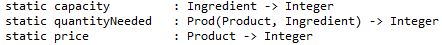
\includegraphics[width=0.8\textwidth]{Immagini/StaticFunction.png}
	\caption{Static functions}
	\label{fig:staticFunc}
\end{figure}
Per esempio la funzione \textit{price} rappresenta un legame costante tra un prodotto e il suo prezzo. 

\subsection{Monitored}
Le funzioni monitored rappresentano degli input che l’utente fornisce alla macchina. Il valore di queste funzioni non è persistente, ma viene ad essere specificato dall’utente per ogni stato tramite tastiera (oppure lette anche da file esterno, come fatto per i test automatici tramite file).
\begin{figure}[h]
	\centering
	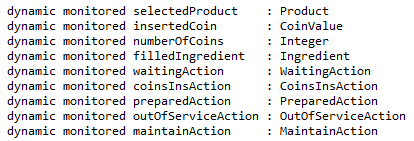
\includegraphics[width=0.8\textwidth]{Immagini/MonitoredFunc.png}
	\caption{Monitored functions}
	\label{fig:monitoredFunc}
\end{figure}
Tra le funzioni monitored figurano le funzioni che richiedono all’utente la scelta tra le azioni disponibili. Inoltre ci sono funzioni con cui l’utente specifica quale moneta, quale prodotto è stato selezionato e, per il manutentore, quale ingrediente è stato rifornito e quante monete ha lasciato nel distributore.

\section{Inizializzazione}
Di default, tutte le funzioni prendono valore undef per quei valori del dominio per cui non sono state esplicitamente definite.	
Perché la macchina inizi a operare in uno stato diverso, più significativo (anche perché raramente la macchina viene definita in modo da poter gestire valori undef), si deve inizializzare la macchina, ovvero definire uno stato iniziale, come fatto in figura ~\ref{fig:initialState}

\begin{figure}[h]
	\centering
	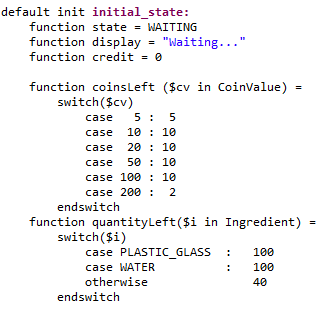
\includegraphics[width=0.8\textwidth]{Immagini/InitialState.png}
	\caption{Inizializzazione}
	\label{fig:initialState}
\end{figure}
In questo caso, lo stato FSM iniziale è quello di attesa, il credito in monete è nullo e la macchina possiede un discreto quantitativo di monete e ingredienti, per poter operare per un certo periodo senza bisogno di manutenzione.

\section{Event management rules e main rule}
Le event management rules si occupano di ricevere le azioni dell’utente e di eseguire (fire) la regola di transizione opportuna. In figura ~\ref{fig:managementRules} c’è un elenco delle regole, la cui struttura è del tutto simile a quella dell’unica regola definita. 

\begin{figure}[h]
	\centering
	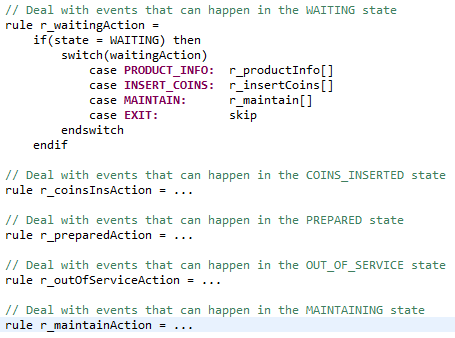
\includegraphics[width=0.8\textwidth]{Immagini/ManagementRule.png}
	\caption{Management rules}
	\label{fig:managementRules}
\end{figure}

La \textit{main rule}, che costituisce l’entry point del programma, controlla per prima cosa che il distributore possa operare, perché non ha finito gli ingredienti (r_selfCheck); questo è possibile grazie al comportamento del blocco sequenziale, che effettua gli update dopo la valutazione di ciascun termine. 

Dopo il controllo, invece, vengono valutate in parallelo le regole di gestione degli eventi: per esse non vi è pericolo di \textit{update inconsistenti} perché ciascuna regola ha una guardia che permette di valutare la regola solo quando la macchina si trova nello stato corretto (ogni regola si applica a un diverso stato, quindi sola una alla volta è “attiva”).

\section{Transition rule}
Ad ogni transizione della FSM, anche se rientrante sullo stesso stato, è associata una regola di transizione, che si occupa di valutare la guardia della transizione e, se questa risulta vera, di eseguire gli update opportuni, andando sostanzialmente ad effettuare un update dello stato.


\section{Simulazione}
La macchina è stata simulata con AsmetaS, sia in modalità interattiva che in modalità batch.
In modalità interattiva è facile scoprire errori sia di transizione di stato FSM sia di update, perché ad ogni update viene mostrato lo stato completo. Tuttavia una simulazione esaustiva è piuttosto lunga, per cui è difficile trovare errori nelle parti di macchina eseguite più raramente.

La modalità random permette di trovare facilmente violazioni inconsistenti: eseguendo una simulazione random con un numero elevato di transizioni (es. 1000) è più probabile coprire anche situazioni poco frequenti o poco naturali per un utente umano.

Per la simulazione batch è stato creato un file di environment testCoffee.env che esegue un tour più o meno completo degli stati e delle transizioni (della FSM).

Per facilitare questo tipo di simulazione è stato introdotta anche l’azione EXIT nel dominio WaitingAction, che è l’unica azione che produce un update set vuoto; è quindi possibile eseguire la simulazione batch con opzione –ne:

\textit{java -jar AsmetaS.jar -ne -env testCoffee.env CoffeeVendingMachine.asm}



	\chapter{Correzione prova}
	\section{EXE 1 - RA}
\begin{itemize}
	\item Pulita disposizione dei record di attivazione: disposti lateralmente, per riprendere la crescita verso il basso dello stack;
	\item Eliminata la colorazione delle variabili che rappresentavano riferimento alla stessa area di memoria (quando si ha passaggio per riferimento, come nel caso della funzione \textit{f(int x, int \&y)} in cui il parametro y viene passato per riferimento);
\end{itemize}

Nella figura ~\ref{fig:ra}, si vede una visione d'insieme (parziale) della correzione dell'esercizio 1, in cui si è seguita una linea di crescita \textit{verticale}, proprio come la memoria stack: in particolare, la \textbf{crescita laterale rappresenta lo sviluppo nel tempo della memoria}, al seguirsi delle varie istruzioni.
\begin{figure}[h]
	\centering
	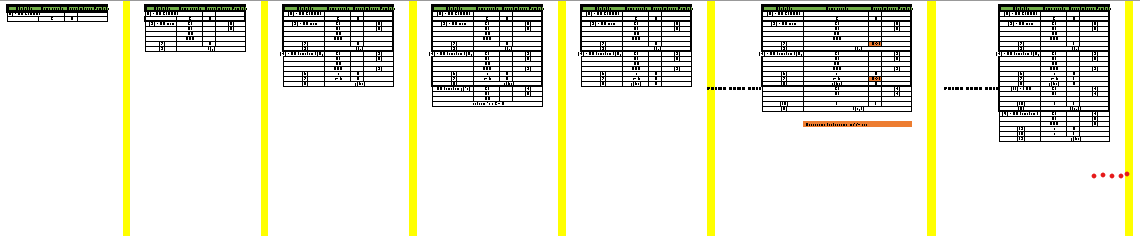
\includegraphics[width=1\textwidth]{Immagini/Partial_RA.png}
	\caption{Parziale soluzione esercizio RA}
	\label{fig:ra}
\end{figure}

\newpage
\section{EXE 2 - C}
Durante la prova, ho optato per risolvere questo esercizio per ultimo: non è stata una scelta felice, poichè sono arrivato dopo 4 ore di prova a cercare di risolvere un problema all'apparenza complicatissimo ma che, con il senno di poi, si è dimostrato risolvibile (con comunque qualche difficoltà).

\subsection{Iterativa}
Per la parte iterativa, durante la prova, non ci sono stati problemi nella stesura di una soluzione.

Nella figura ~\ref{fig:sppIt}, si vede come siamo andati a settare uno spazio di memoria dinamico, con l'istruzione \textit{malloc} di lunghezza sensata: infatti, a tutti i numeri pari da 0 a N ($N/2$) abbiamo aggiunto uno spazio necessario per aggiungere il \textit{numero terminatore} (in questo caso 1).

Il risultato poi è stato popolato con accesso tramite deferenziazione (riga 21).
\begin{figure}[h]
	\centering
	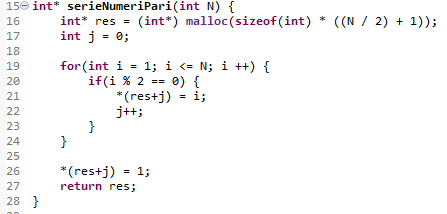
\includegraphics[width=0.6\textwidth]{Immagini/SerieNumeriPariIt.png}
	\caption{Serie numeri pari Iterativa}
	\label{fig:sppIt}
\end{figure}


\subsection{Ricorsiva senza tail}
Sicuramente questa soluzione richiedeva uno sforzo maggiore.

Riprovando a casa, sono arrivato ad una soluzione, riportata in figura ~\ref{fig:sppRecNoTail}.

\begin{figure}[h]
	\centering
	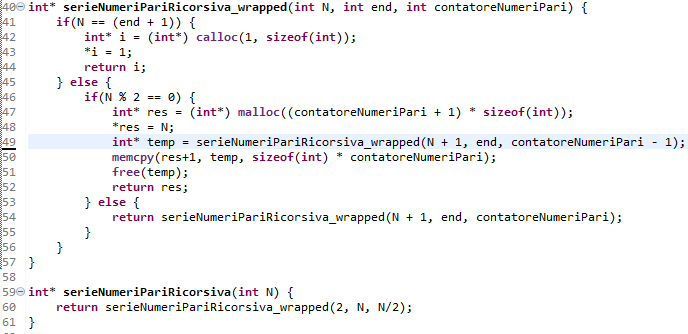
\includegraphics[width=0.6\textwidth]{Immagini/SerieNumeriPariRecNoTail.png}
	\caption{Serie numeri pari ricorsiva senza tail [operazioni di debug omesse]]}
	\label{fig:sppRecNoTail}
\end{figure}

\begin{figure}[h]
	\centering
	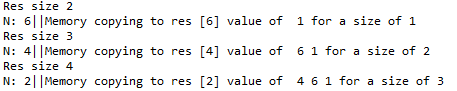
\includegraphics[width=0.6\textwidth]{Immagini/SerieNumeriPariRecNoTailDebug.png}
	\caption{Serie numeri pari ricorsiva senza tail - debug print}
	\label{fig:sppRecNoTailLog}
\end{figure}

Rispetto alla prova, ho apportato questi cambiamenti:
\begin{itemize}
	\item Ho inserito una funzione wrapper, per nascondere all'utente il fatto che la scansione dei numeri parta da 2 (ho scartato lo 0 e l'1 che sono dispari) arrivando fino a N, così da ritornare un risultato che sia in ordine crescente;
	\item \textit{contatoreNumeriPari} è utilizzato per poter sfruttare al meglio il comando di memcpy, in maniera tale da copiare/allocare solamente la quantità di memoria necessaria
	\item Il risultato è salvato in una variabile temporanea per poterne poi fare il free: questo fa si che i valori numerici vengano ananlizzati in maniera decrescente (prima annido le chiamate per valori decrescenti, e poi analizzo i risultati in maniera decrescente)
	\item La condizione d'uscita si ha quando raggiungo il valore successivo al valore passato in input dall'utente (end + 1);
	\item Essendo che salvo il risultato in una variabile temporanea (riga 49), per poterne poi fare il free, l'analisi dei risultati sarà effettuato in ordine inverso: è per questo motivo che il contatore dei numeri pari parte dal valore completo (N/2) e decresce (e quindi i valori da copiare dovranno essere 1, e via via crescenti);
\end{itemize}

\subsection{Ricorsiva CON tail}
La versione tail è stata leggermente modificata: anche qui, come nella versione non tail, ho inserito una funzione wrapper, per nascondere all'utente il comportamento a basso livello della funzione.

Nello specifico anche qui faccio partire il conteggio daa 2, per farlo concludere quando raggiunge il valore (end + 1).

\section{EXE 3 - C++ distruttore}
Il distruttore è il metodo duale del costruttore: esso serve principalmente ad eliminare gli oggetti
della memoria, andando quindi a liberare spazio in memoria.

Il distruttore viene chiamato automaticamente dal compliatore quando la variabile esce dal suo scope.
Questa eliminazione automatica però non avviene per i puntatori: quindi se ho un puntatore (allocato tramite la funzione malloc) sarà necessario che sia invocato esplicitamenteun comando di free per evitare un memory leakage.

Nel caso di utilizzi di sottoclassi è sempre meglio dichiarare il distruttore virtual così che chiami tutti i distruttori delle superclassi (dalla sottoclasse e poi fino alla superclasse)
\section{EXE 4 - Opachi}

Rispetto alla soluzione proposta in prova, sono andato a snellire il metodo \textit{somma} utilizzando l'init \textit{make} come si vede in figura ~\ref{fig:makeSomma}.

\begin{figure}[h]
	\centering
	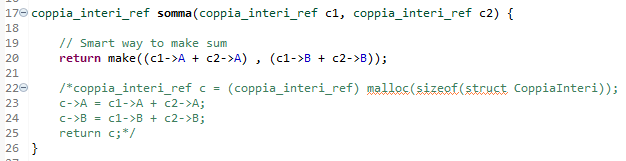
\includegraphics[width=0.6\textwidth]{Immagini/makeSommaOpachi.png}
	\caption{Metodo \textit{make}}
	\label{fig:makeSomma}
\end{figure}

\section{EXE 5 - Visitor}
Durante la prova avevo inserito il Visitor anche per le \textit{FigureGeometriche} astratte: questo perchè nel metodo \textit{calcolaMax} andavo a chiamare la funzione \textit{visit} invece che \textit{accept}, il chè quindi mi ha portato ad inserire il visitor anche per la classe astratta.

Ho corretto quindi il metodo \textit{calcolaMax} come si vede in figura ~\ref{fig:calcolaMax}.

\begin{figure}[h]
	\centering
	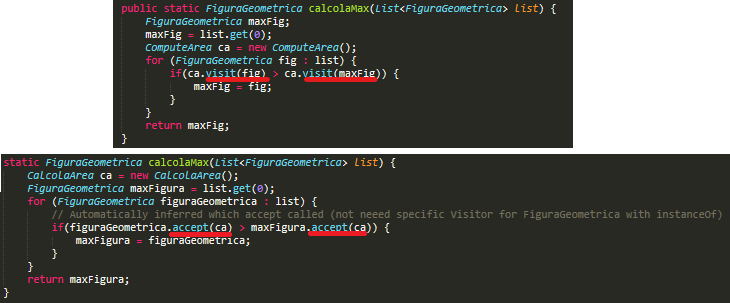
\includegraphics[width=0.6\textwidth]{Immagini/calcolaMax.png}
	\caption{Confronto tra metodi calcolaMax (prova sopra e correzione sotto)}
	\label{fig:calcolaMax}
\end{figure}

Ho inoltre corretto anche la segnatura del metodo.
\section{EXE 6 - Scala}
Nella correzione della prova di Scala sono andata ad inserire il wrapper, come si vede in figura ~\ref{fig:scalaWrap}: ho sfruttato la possibilità che Scala offre di definire funzioni \textit{inline}.

\begin{figure}[h]
	\centering
	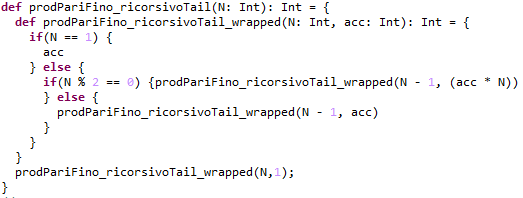
\includegraphics[width=0.6\textwidth]{Immagini/scalaWrap.png}
	\caption{Wrap in Scala}
	\label{fig:scalaWrap}
\end{figure}

Ho inoltre anche aggiunto l'utilizzo delle \textit{High Order Functions}: nella specifico ho inserito una \textit{HOF} per andare a generalizzare il criterio della funzione: nello specifico, con questa \textit{HOF} si può andare a settare il valore per cui poi sommeremo solamente i numeri divisibili per tale valore.

Per esempio, nel main di prova, ho settato il criterio pari a 5: in questo modo sommeremo tutti i numeri divisibili per 5.

\end{document}
